\documentclass[]{tukethesis}
%% -------------------------------------------------------------------------
%% UTF-8 encoding used. Use pdfcslatex to compile your document
%% Tukethesis Class for Win XP and GNU/Linux
%% -------------------------------------------------------------------------
\usepackage[utf8]{inputenc}
%\usepackage[T1]{fontenc}
\usepackage{lmodern,cmap}
%\usepackage{english}
\renewcommand{\figurename}{Fig.}
\renewcommand{\tablename}{Tab.}
\renewcommand{\refname}{Bibliography}
\renewcommand{\listfigurename}{List of Figures}
\renewcommand{\listtablename}{List of Tables}
\renewcommand{\contentsname}{Contents}
%%
%\usepackage{cite}
\usepackage[english]{babel}
\usepackage{latexsym}
\usepackage[strings]{underscore}
\usepackage{dcolumn} % alignment on a 'decimal point' in tabular mode
\usepackage{hhline}
\usepackage{amsfonts}
\usepackage{amsmath}
\usepackage{amssymb}
%\usepackage{mhchem}
\usepackage{nicefrac} % nice fractions
\usepackage{upgreek} % e.g. $\upmu\mathrm{m}$ type micrometer (mu)
\usepackage[final]{showkeys}%color%notref%notcite%final
\usepackage[noprefix]{nomencl}
\makeglossary % command to make *.glo file
\usepackage{parskip}%
\usepackage{caption}
\usepackage{color}
\usepackage{xcolor}
\usepackage{subfig}
% Code rendering
\usepackage{listings, listings-rust}
\renewcommand{\lstlistingname}{Listing}%
\definecolor{GrayCodeBlock}{RGB}{249,249,249}
\definecolor{BlackText}{RGB}{110,107,94}
\definecolor{RedTypename}{RGB}{182,86,17}
\definecolor{GreenString}{RGB}{96,172,57}
\definecolor{PurpleKeyword}{RGB}{184,84,212}
\definecolor{GrayComment}{RGB}{170,170,170}
\definecolor{GoldDocumentation}{RGB}{180,165,45}

% Rust
\lstdefinelanguage{rust}
{
	columns=fullflexible,
	keepspaces=true,
	frame=single,
	framesep=5pt,
	framerule=0pt,
	framexleftmargin=35pt,
	framexrightmargin=4pt,
	framextopmargin=5pt,
	framexbottommargin=3pt,
	xleftmargin=35pt,
	xrightmargin=4pt,
	backgroundcolor=\color{GrayCodeBlock},
	basicstyle=\ttfamily\color{BlackText}\linespread{0.9}\footnotesize,
	numbers=left,                    
	numbersep=5pt,    
	numberstyle=\color{GrayComment}\footnotesize,
	breakatwhitespace=false,         
	breaklines=true,                 
	captionpos=b,                         
	numbers=left,                    
	numbersep=20pt,           
	showspaces=false,                
	showstringspaces=true,
	showtabs=false,                  
	tabsize=2,
	keywords={
		true,false,
		unsafe,async,await,move,
		use,pub,crate,super,self,mod,
		struct,enum,fn,const,static,let,mut,ref,type,impl,dyn,trait,where,as,
		break,continue,if,else,while,for,loop,match,return,yield,in
	},
	keywordstyle=\color{PurpleKeyword},
	ndkeywords={
		bool,u8,u16,u32,u64,u128,i8,i16,i32,i64,i128,char,str,
		Self,Option,Some,None,Result,Ok,Err,String,Box,Vec,Rc,Arc,Cell,RefCell,HashMap,BTreeMap,macro_rules,af,arrayfire
	},
	ndkeywordstyle=\color{RedTypename},
	comment=[l][\color{GrayComment}\slshape]{//},
	morecomment=[s][\color{GrayComment}\slshape]{/*}{*/},
	morecomment=[l][\color{GoldDocumentation}\slshape]{///},
	morecomment=[s][\color{GoldDocumentation}\slshape]{/*!}{*/},
	morecomment=[l][\color{GoldDocumentation}\slshape]{//!},
	morecomment=[s][\color{RedTypename}]{\#![}{]},
	morecomment=[s][\color{RedTypename}]{\#[}{]},
	stringstyle=\color{GreenString},
	string=[b]"
	emph={int,char,double,float,unsigned},
	emphstyle={\color{blue}}]
}

%C++
\lstdefinelanguage{cpp}
{
	columns=fullflexible,
	keepspaces=true,
	frame=single,
	framesep=5pt,
	framerule=0pt,
	framexleftmargin=20pt,
	framexrightmargin=4pt,
	framextopmargin=5pt,
	framexbottommargin=3pt,
	xleftmargin=20pt,
	xrightmargin=4pt,
	backgroundcolor=\color{GrayCodeBlock},
	basicstyle=\footnotesize\linespread{0.9}\color{BlackText},
	numbers=left,                    
	numbersep=5pt,    
	breakatwhitespace=false,         
	breaklines=true,                 
	captionpos=b,                         
	numbers=left,                    
	numbersep=5pt,      
	numberstyle=\footnotesize,     % numbers size        
	showspaces=false,                
	showstringspaces=true,
	showtabs=false,                  
	tabsize=2,
	keywords={
		true,false,
		unsafe,async,await,move,
		use,pub,crate,super,self,mod,
		struct,enum,fn,const,static,let,mut,ref,type,impl,dyn,trait,where,as,
		break,continue,if,else,while,for,loop,match,return,yield,in,array
	},
	keywordstyle=\color{PurpleKeyword},
	ndkeywords={
		bool,u8,u16,u32,u64,u128,i8,i16,i32,i64,i128,char,str,unsigned,
		Self,Option,Some,None,Result,Ok,Err,String,Box,Vec,Rc,Arc,Cell,RefCell,HashMap,BTreeMap,
		macro_rules
	},
	ndkeywordstyle=\color{RedTypename},
	comment=[l][\color{GrayComment}\slshape]{//},
	morecomment=[s][\color{GrayComment}\slshape]{/*}{*/},
	morecomment=[l][\color{GoldDocumentation}\slshape]{///},
	morecomment=[s][\color{GoldDocumentation}\slshape]{/*!}{*/},
	morecomment=[l][\color{GoldDocumentation}\slshape]{//!},
	morecomment=[s][\color{RedTypename}]{\#![}{]},
	morecomment=[s][\color{RedTypename}]{\#[}{]},
	stringstyle=\color{GreenString},
	string=[b]"
}

% C#
\lstdefinelanguage{csharp}
{
	columns=fullflexible,
	keepspaces=true,
	frame=single,
	framesep=5pt,
	framerule=0pt,
	framexleftmargin=35pt,
	framexrightmargin=4pt,
	framextopmargin=5pt,
	framexbottommargin=3pt,
	xleftmargin=35pt,
	xrightmargin=4pt,
	backgroundcolor=\color{GrayCodeBlock},
	basicstyle=\ttfamily\color{BlackText}\linespread{0.9}\footnotesize,
	numbers=left,                    
	numbersep=5pt,    
	numberstyle=\color{GrayComment}\footnotesize,
	breakatwhitespace=false,         
	breaklines=true,                 
	captionpos=b,                         
	numbers=left,                    
	numbersep=20pt,           
	showspaces=false,                
	showstringspaces=true,
	showtabs=false,                  
	tabsize=2,
	keywords={
		true,false,
		unsafe,async,await,move,
		use,pub,crate,super,self,mod,
		struct,enum,fn,const,static,let,mut,ref,type,impl,dyn,trait,where,as,
		break,continue,if,else,while,for,loop,match,return,yield,in
	},
	keywordstyle=\color{PurpleKeyword},
	ndkeywords={
		bool,u8,u16,u32,u64,u128,i8,i16,i32,i64,i128,char,str,
		Self,Option,Some,None,Result,Ok,Err,String,Box,Vec,Rc,Arc,Cell,RefCell,HashMap,BTreeMap,macro_rules,af,arrayfire
	},
	ndkeywordstyle=\color{RedTypename},
	comment=[l][\color{GrayComment}\slshape]{//},
	morecomment=[s][\color{GrayComment}\slshape]{/*}{*/},
	morecomment=[l][\color{GoldDocumentation}\slshape]{///},
	morecomment=[s][\color{GoldDocumentation}\slshape]{/*!}{*/},
	morecomment=[l][\color{GoldDocumentation}\slshape]{//!},
	morecomment=[s][\color{RedTypename}]{\#![}{]},
	morecomment=[s][\color{RedTypename}]{\#[}{]},
	stringstyle=\color{GreenString},
	string=[b]"
	emph={int,char,double,float,unsigned},
	emphstyle={\color{blue}}]
}
%%%%%%%
\usepackage{bm}
%
\usepackage{mathptmx}      % use Times fonts if available on your TeX system
%
% insert here the call for the packages your document requires
%\usepackage{natbib}
\usepackage[hyphens]{url}
\urlstyle{same}
\usepackage{etoolbox}

% Quotes
\makeatletter
%\renewcommand{\@chapapp}{}% Not necessary...
\newenvironment{chapquote}[2][2em]
{\setlength{\@tempdima}{#1}%
	\def\chapquote@author{#2}%
	\parshape 1 \@tempdima \dimexpr\textwidth-2\@tempdima\relax%
	\itshape}
{\par\normalfont\hfill--\ \chapquote@author\hspace*{\@tempdima}\par\bigskip}
\makeatother

%%
%\usepackage[dvips]{graphicx}
%\DeclareGraphicsExtensions{.eps, .mps}
\usepackage[pdftex]{graphicx}
\DeclareGraphicsExtensions{.pdf,.png,.jpg,.mps}
%\usepackage[os=mac, mackeys=symbols]{menukeys}
\graphicspath{{figures/}} % directory for figures
%%
%% numerical citations (vancouer style)
%\usepackage[numbers]{natbib}
%%
%% author-year citations (harvard style) -- prefered !!!
\usepackage{natbib}
%\citestyle{chicago}
% -----------------------------------------------------------------
%% tlač !!!
\usepackage[pdftex,unicode=true,bookmarksnumbered=true,
bookmarksopen=true,pdfmenubar=true,pdfview=Fit,linktocpage=true,
pageanchor=true,bookmarkstype=toc,pdfpagemode=UseOutlines,
pdfstartpage=1]{hyperref}

\hypersetup{%
baseurl={http://www.tuke.sk/sevcovic},
pdfcreator={pdfcsLaTeX},
pdfkeywords={Visualization, Virtual Reality},
pdftitle={Design and implementation of modern methods of modeling and control of technological objects and processes},
pdfauthor={Ing. Michal Tak\'ač},
pdfsubject={Dissertation Thesis}
colorlinks=true,       % false: boxed links; true: colored links
citebordercolor=1 1 1,
breaklinks=true,
linkcolor=blue,          % color of internal links (change box color with linkbordercolor)
citecolor=blue,        % color of links to bibliography
filecolor=blue,      % color of file links
urlcolor=blue           % color of external links
} 
%% -----------------------------------------------------------------
%% START YOUR THESIS
%% -----------------------------------------------------------------
%%

\masterthesis{Dissertation Thesis}


\author{Michal Takáč}
\title{Design and Implementation of Modern Methods for Modeling and Control of Technological Objects and Processes}
\subtitle{}
\abstrakte{Text abstraktu v~svetovom jazyku je potrebný pre integráciu
do medzinárodných informačných systémov. Ak nie je možné cudzojazyčnú
verziu abstraktu umiestniť na jednej strane so slovenským abstraktom,
je potrebné umiestniť ju na samostatnú stranu (cudzojazyčný abstrakt
nemožno deliť a~uvádzať na dvoch strabách).}
\keywords{Mathematical modeling, Simulation, Visualization, Virtual Reality}
\degree{PhD.}
\university{Technical University of Košice}
\faculty{Faculty of Mining, Ecology, Process Control and Geotechnologies}
\facultyabbr{FBERG}
\department{Institute of Control and Informatization of Production Processes}
\departmentabbr{URIVP}
\fieldofstudy{Cybernetics}
\studyprogramme{Process Control}
\supervisor{prof.~Ing.~Ivo~Petráš, DrSc.}
%\consultanta{}
%\consultantb{}
\dateofsubmission{April. 1. 2021} 
\town{Košice}
\abstrakt{Abstrakt je povinnou súčasťou každej práce. Je výstižnou
charakteristikou obsahu dokumentu. Nevyjadruje hodnotiace stanovisko
autora. Má byť\/ taký informatívny, ako to povoľuje podstata práce.
Text abstraktu sa píše ako jeden odstavec. Abstrakt neobsahuje odkazy
na samotný text práce. Mal by mať\/ rozsah 250 až 500 slov. Pri
štylizácii sa používajú celé vety, slovesá v činnom rode a tretej
osobe. Používa sa odborná terminológia, menej zvyčajné termíny,
skratky a~symboly sa pri prvom výskyte v texte definujú.}
\klucoveslova{Matematické modelovanie, Simulácia, Vizualizácia, Virtuálna realita}

\begin{document}
\renewcommand\theHfigure{\theHsection.\arabic{figure}}
\renewcommand\theHtable{\theHsection.\arabic{table}}
\bibliographystyle{dcu}
%% input the 'First page of the Thesis'
\firstpage

%% input the 'Title page of the Thesis'
\titlepage

%% input the 'Metadatasheet of the Thesis'
%\metadatasheet

%\errata % begin the 'Errata' 
%Ak je potrebné, autor na tomto mieste opraví chyby, ktoré našiel
%po vytlačení práce. Opravy sa uvádzajú takým písmom, akým je napísaná
%práca. Ak zistíme chyby až po vytlačení a zviazaní práce, napíšeme
%erráta na samostatný lístok, ktorý vložíme na toto miesto. Najlepšie je
%lístok prilepiť\/ \citep{kat}.
%
%Forma:
%
%\tabcolsep=10pt
%\begin{table}[!hb]
%	\centering
%	\begin{tabular}{|c|c|c|c|}\hline
%Strana & Riadok & Chybne & Správne \\\hline\hline
%12 & 6 & publikácia & prezentácia \\\hline
%22 & 23 & internet & intranet \\\hline
%& & & \\\hline
%& & & \\\hline
%	\end{tabular}
%\end{table}
%\kerrata

\abstrakte % Abstract in English

\abstrakt % Abstract in Slovak

\endabstract % end of the Abstracts page

%% input the 'Assign of the Thesis'
\assignthesis

%% input the 'Declaration' of the author
\declaration
% I hereby declare that this thesis is my own work and effort. Where
% other sources of information have been used, they have been
% acknowledged.
%%
% Niektorí autori metodických príručiek o~záverečných prácach sa
% nazdávajú, že takéto vyhlásenie je zbytočné, nakoľko povinnosť
% vypracovať záverečnú prácu samostatne, vyplýva študentovi zo zákona
% a na  autora práce sa vzťahuje autorský zákon.

\acknowledgement % begin the 'Acknowledgement'
I would like to express my sincere thanks to my supervisor Prof.~Ing.~Ivo~Petráš, DrSc., the main Supervisor, for his constant, and constructive guidance
throughout the study. To all other who gave a hand, I say thank you
very much.
\endacknowledgement

\preface % begin the 'Preface'
Predhovor...
\endpreface

\thispagestyle{empty}
\tableofcontents
\newpage

\thispagestyle{empty}
%\addcontentsline{toc}{section}{\numberline{}List of Figures}
\listoffigures
\newpage

\thispagestyle{empty}
%\addcontentsline{toc}{section}{\numberline{}List of Tables}
\listoftables
\newpage

\thispagestyle{empty}
%\addcontentsline{toc}{section}{\numberline{}List of Symbols and
%Abbreviations}
\printglossary % input the 'List of Symbols and Abbreviations'
\newpage

%\addcontentsline{toc}{section}{\numberline{}List of Therms}
\listofterms % begin the 'List of Therms'

\begin{description}
	\item[LBM] - Lattice Boltzmann Method.
	\item[LBE] - Lattice Boltzmann Equation.
	\item[DF] - Distribution Function.
	\item[GPU] - Graphics Processing Unit.
	\item[GPGPU] - General-Purpose Computing on Graphics Processing Unit.
	\item[D2Q9] - Two-dimensional lattice stencil with 9 discrete velocity directions in each node.
	\item[D3Q27] - Three-dimensional lattice stencil with 27 discrete velocity directions in each node.
	\item[JIT] - Just-In-Time compilation.
	\item[API] - Application Programming Interface.
\end{description}

\endlistofterms
%
\section{Introduction}

The objective of process control is to keep key process-operating parameters within nar- row bounds of the reference value or setpoint. Controllers are used to automate a human function in an effort to control a variable. A basic controller can keep an individual loop on an even point, so long as there is not too much disruption. Complex processes like ones in metallurgy might employ dozens or even hundreds of such controllers, but keep- ing an eye on the big picture was, until not so long ago, a human process.
Although a device was used to automate a human function in an effort to control a vari- able, there was no sense of what the process was doing overall. A basic controller could keep an individual loop on an even keel, more or less, so long as there was not too much disruption. Complex processes might employ dozens or even hundreds of such controllers, each with its performance displayed on a panel board, but keeping an eye on the big picture was still a human process.

When distributed control system (DCS) platforms were introduced in the 1970s, they sim- plified the mechanics of the panel board, but did not do much to improve its capabilities. Big-picture analysis was still largely a human responsibility. Sure, getting beyond the technical constraints of pneumatic field devices with their troublesome compressed air tubing made it easier to install more instruments and actuators, but the basic control con- cepts did not really change. Any movement to advanced process control (APC) and other forms of control optimization were still in their infancy. Process automation capable of supporting APC had to encompass many technologies and techniques. It was character- ized by incorporating many more input data points into algorithms and orchestrating more complex sequences.

The transition to process automation and advanced process control (APC) was empowered by being able to create an all-encompassing platform capable of coordinating more than single loops or small cascade groups. One major advantage of newer platforms is the abil- ity to optimize a process to suit the owner’s specific economic goals based on any number of desired outcomes. The process automation system can operate the plant to minimize energy consumption, maximize output, and deliver specific product quality attributes.

Implementing such systems is challenging. During the initial design phase of a control system upgrade or a new installation, it is far too easy to focus just on process funda- mentals, and never get beyond considering desired steady-state conditions. Automation system upgrades and new installations can therefore miss opportunities to engage with process and automation technology experts capable of uncovering better ways of doing things. Many capabilities of modern process automation systems are still underutilized in most process plants. Far fewer companies use APC as effectively as they could, even though basic APC technologies have been around for decades.

\section{Basic Oxygen Furnace}

The oxygen converter process (LD/BOF and its derivatives) is a refinement step in the pro- duction of steel from ore. The main purpose of the process is to remove excess carbon from the pig iron produced in the blast furnace. The main feature of the process is to add oxygen through a top lance, in order to remove unwanted impurities through oxidation. It is the main method of carbon and low alloy steelmaking, annual production approaching to 60\% of total crude steel production \cite{Jalkanen2006}. BOF is a widely preferred and effective steelmaking method due to its high productivity and considerably low production cost \cite{Wang2010}. LD/BOF process consists of these subprocesses:

\begin{enumerate}
\item Charging slag
\item Charging hot metal
\item Oxygen blowing and addition of slagging and alloying additives 4. Measurement of steel temperature and composition
\item Tapping of steel
\item Tapping of slag
\end{enumerate}

The first commercial operation of steelmaking with oxygen top blowing in the converter was in the early 1950s at Linz and Donawitz (Austria). This manner of steelmaking be- came known as Linz-Donawitz or LD process. For many years now, most of the steel has been made by top oxygen blowing for which different names are given. For example, in European steel plants the process is still called LD; in the UK, BOS (basic oxygen steel- making); in the Far East and America, BOF (basic oxygen furnace), with the exception of U.S. Steel where it is called basic oxygen process \cite{Turkdogan1996}.

\begin{figure}[!ht]
	\label{fig:bof-single}
	\centering
	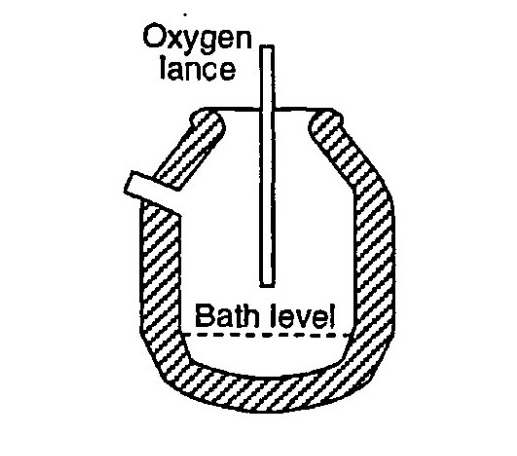
\includegraphics[width=0.5\textwidth]{figures/bof-single.jpg}
	\caption{Production of steel in the converter with top-blown oxygen (LD/BOF) \citep{Turkdogan1996}.}
\end{figure}

In modern steel mills about 300 tons of steel are produced within a 30-40 minute cycle. Various additives are added during the process to adapt the steel quality and slag formation. The converter furnace is inclined during charging and tapping. The converter has a vertical position during oxygen blowing. The changes in the position of the converter during the individual elementary processes are shown in the figure \ref{fig:convertor-phases}.


\begin{figure}[!ht]
	\label{fig:convertor-phases}
	\centering
	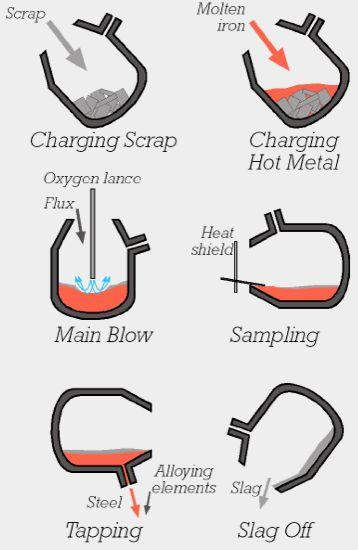
\includegraphics[width=0.4\textwidth]{figures/convertor-phases.jpg}
	\caption{Representation of elementary processes in LD converter.}
\end{figure}

Depending on local operating conditions, availability of scrap, blast furnace iron and the ex- tent of hot metal pretreatment, the metallic charge (LD/BOF, Q-BOP) is $75$ to $95\%$ pig iron and the remainder is steel scrap. The types of scrap used are usually those produced in a steel mill: sheet scrap, damaged molds, bimetallic cans etc. \citep{Turkdogan1996}.

Oxygen is blown at a high speed (up to twice the speed of sound) on the surface of the metal bath in the converter and so-called hot area is formed in the region where the oxygen stream hits the surface. The oxidation products dissolve in the slag, with the exception of carbon monoxide, which passes through the slag layer and forms the major component of the converted gas. The oxidation intensity of the individual elements depends on their chemical affinity for oxygen. Carbon oxidation is one of the most important processes. Carbon is oxidized in the metal during the steelmaking process by the influence of oxygen, in particular on \ce{CO} and partly on \ce{CO2}, depending on the reactions

\begin{equation}
	\ce{ C + 1/2 O2 -> 2CO }
\end{equation}

\begin{equation}
	\ce{ C + O2 -> CO2 }
\end{equation}

Manganese is oxidized to \ce{MnO}

\begin{equation}
	\ce{ Mn + 1/2 O2 -> MnO },
\end{equation}

Phosphorus is undesirable in steel and oxidizes to \ce{P2O5}

\begin{equation}
	\ce{ 2P + 5/2 O2 -> P2O5 }.
\end{equation}

Sulphur is a harmful element and passes into the slag in the form of \ce{CaS} based on the reaction of \ce{CaO}

\begin{equation}
	\ce{ CaO + MnS -> CaS + MnO }
\end{equation}

whereby \ce{MnS} is formed by reaction

\begin{equation}
	\ce{ Mn + S -> MnS }
\end{equation}

and sulphur also goes out in the form of gas as \ce{SO2}

\begin{equation}
	\ce{ S + O2 -> SO2 }.
\end{equation}

Silicon has a high affinity for oxygen, so it is easily oxidized to form \ce{SiO2}

\begin{equation}
	\ce{ Si + O2 -> SiO2 }.
\end{equation}

In the initial stages of blowing, most of the silicon oxidizes to form a slag of low basicity - the composition of the metal and slag changes TODO: DOPLNIT ZDROJ!!!. 

An intense oxygen flow induces fluid flows in the iron bath, forcing the highly oxidized metal and the molten oxidation products from the iron bath surface to penetrate into the bath, where they react with the ``fresh" hot metal with a high content of impurities and therefore loss of iron in the form of \ce{FeO} and \ce{Fe2O3}should also be considered:

\begin{equation}
	\ce{ Fe + 1/2 O2 -> FeO }
\end{equation}

\begin{equation}
	\ce{ 2Fe + 3/2 O2 -> Fe2O3 }.
\end{equation}

This oxygen stream and gas bubbles generated in the bath bring portions of the iron melt to the slag. The heat generated by the highly exothermic oxidation reactions is consumed by heating and melting the feed materials, heating the iron bath, slag and carbon oxides that are formed during the oxidation of the carbon and are partially lost to the environment during the blowing process.

The resulting \ce{SiO2} passes into the slag as \ce{2CaO.SiO2} according to the equation

\begin{equation}
	\ce{ SiO2 + 2CaO -> 2CaO.SiO2 }
\end{equation}

and additionally, \ce{P2O5} passes into the slag as \ce{3CaO.P2O5} according to the equation \cite{sprava2017}

\begin{equation}
	\ce{ P2O5 + 3CaO = 3CaO.P2O5 }
\end{equation}

Circulation in the iron bath caused by the flow of oxygen, rising gas bubbles and purging of inert gas through the lower tubes in converters with combined blowing type transports minor iron melt components (C, Si, Ti, Mn, P, V, etc.) to the upper bath layers \citep{Jalkanen2006}.

\begin{figure}[!ht]
	\label{fig:ld-convertor-processes-graphical}
	\centering
	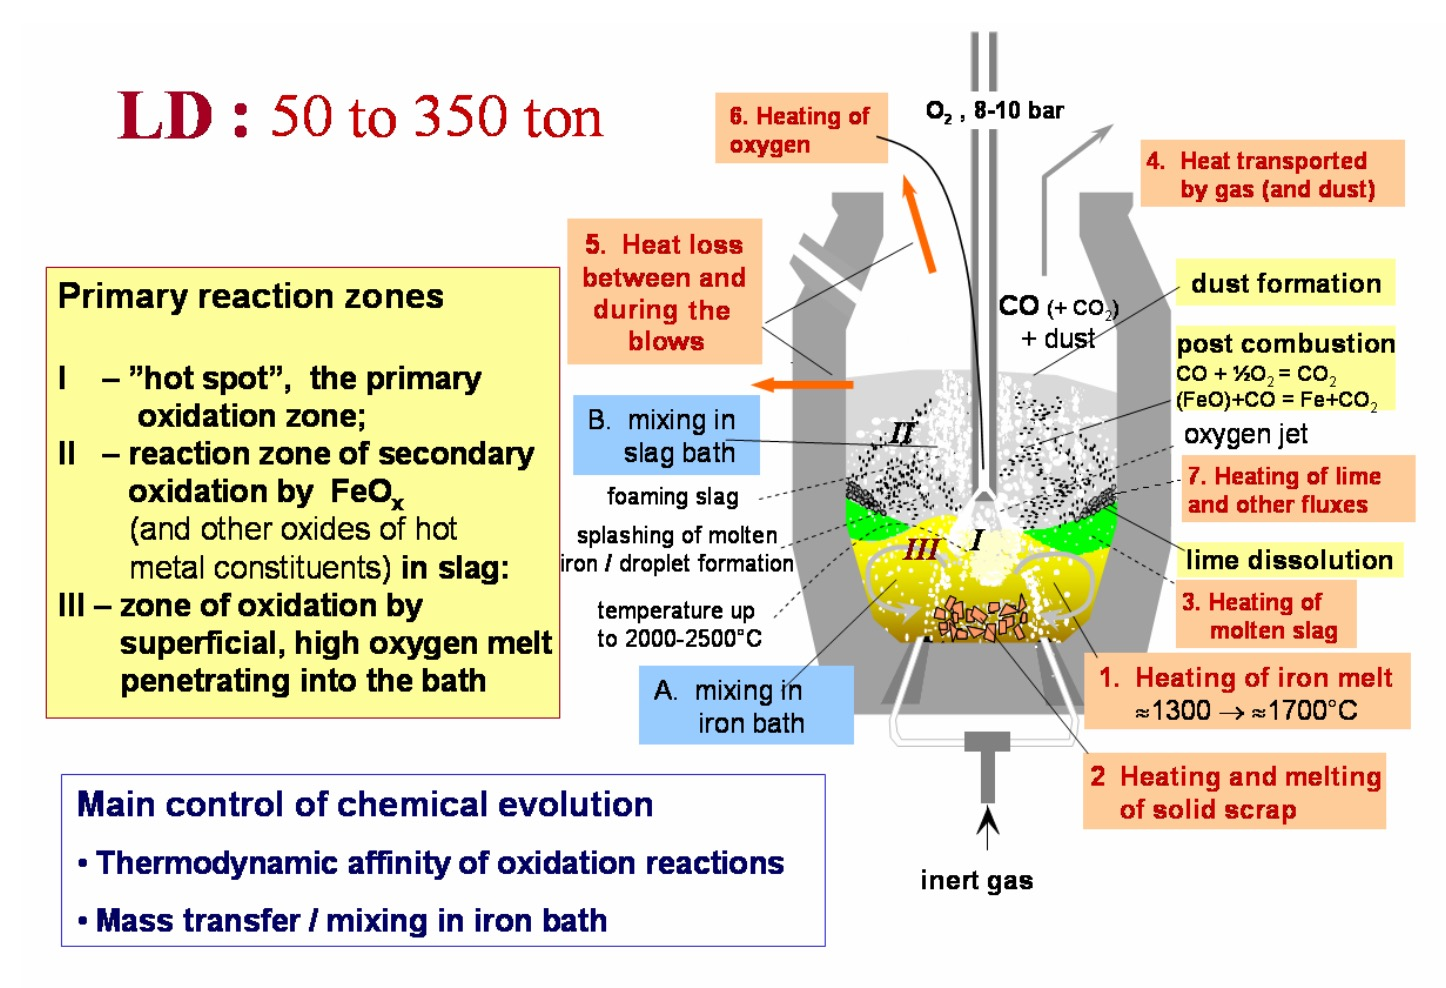
\includegraphics[width=0.8\textwidth]{figures/ld-convertor-processes-graphical.jpg}
	\caption{Chemical and thermal processes in LD converter \citep{Jalkanen2006}.}
\end{figure}

In order to monitor and control the process, different measuring systems can be employed to give feedback to either the operator or directly to existing system for automated control. These measurements can be either direct or indirect as well as with or without time delays. The real-time information on the process state can be obtained from a number of sensors, e.g. off-gas flow rate from venturi; off-gas temperature with temperature sensors; indication of changes in slag level from sound level measurement with microphone, accelerometer on lance or vessel or lance elongation sensor; pressure difference with ambient pressure with hood pressure sensor, etc.

All these signals can, in principle, be used for closed-loop control. Changes in lance height are easier to measure as well as set and therefore preferable to use in a closed- loop control system. Oxygen gas flow rate should not be changed more than approximately $\pm5\%$ since the nozzle is designed for a specific flow rate \citep{Widlund1998}.

TODO: DOPLNIT SCHEMU RIADIACEHO SYSTEMU

Different operators apply different rules for deciding when to stop the blowing of oxygen. These operator induced irregularities make it difficult to achieve production disturbances. The converter process is only one link in a chain of unit operations from raw materials to final product. Therefore, production disturbances can change process conditions. For example, poor blast furnace performance might lead to insufficient hot metal supply or even production disruptions. Under these circumstances, more metal scrap and fuel should be used instead of hot metal to uphold production volumes. Logically, this implies changes in blowing practice \citep{Widlund1998}.

\section{Computer-aided Mathematical Modeling and Numerical Simulation}

The motivation for using computer simulations to investigate metallurgical processes is two-fold. First, it enables design changes to be tested before building a prototype, which naturally leads to a lower total design cost. Second, it makes it possible to investigate phenomena that cannot easily be measured or observed in the process. Even a seemingly simple operation such as the continuous measurement of the temperature during the decarburization process is difficult due to the very high temperatures in the process and generally harsh conditions prevailing in the steel plants (Ersson and Tilliander; 2018).
In metallurgy, simulating linear and non-linear processes that we encounter in steelmak- ing by creating mathematical models is of great importance. Since first attempts to use mathematical techniques for the simulation and optimization of large scale metallurgical operations (Ray et al.; 1973), various numerical methods were implemented as algorithms and used to simulate phenomena in steelmaking processes. One class of such methods is Monte Carlo, which is useful for simulating systems with many coupled degrees of freedom such as fluids.

Modern fluid mechanics problems would be impossible to solve without use of Compu- tational Fluid Dynamics (CFD), since the scope of analytical solutions to fundamental equations of fluid mechanics is very limited and, once a more difficult geometry is en- countered, we usually have to choose a given numerical method for obtaining a solution. CFD encompasses a wide spectrum of numerical methods used for solving complex three-dimensional (3D) and time-dependent flow problems (Rapp; 2017). Since early pioneering work in the metallurgical field done by Szekely et al. (1977), the cost of performing computer simulations has decreased over the last few decades, while the available processing power has increased. Most of the processors and processing units that are currently developed and produced have several cores that can execute instructions in parallel. Thus, the processing power available to a CFD software also depends on the capability of the software to execute in parallel. A study by Ersson and Tilliander (2018) of the last two decades of metallurgical CFD simulations reveals huge improvements on the type of phenomena that can be explored and we will see this trend is continuing thanks to improvements in both the available processing power and the avail- able algorithms. Therefore CFD found its way into numerous studies in steelmaking, where these methods proved useful in demonstrating the hidden and significant proper- ties. However, its use in the steel industry may not be as integrated as in the aero and automotive industries, in which the development of new designs is of key importance. The major difference between aero and metallurgical industries is that the metallurgical industries almost always deal with multiphase systems at elevated temperatures and that the motivation of modeling is mainly process optimization. With a continuing development in multiphase models as well as in reacting flow modeling, the continued usefulness of CFD in metallurgy remains clear.

In LD/BOF process, different chemical reactions among oxygen, slag, and molten iron in oxygen converter, in combination with vigorous stirring process to promote slagging, dephosphorization, decarbonization, heating of molten steel, and homogenization of steel composition and temperature, determines the final properties of steel. The objective of the oxygen converter is to refine molten iron to crude steel through oxidization to achieve a specified temperature and chemical composition at the end blow. Failure to do this leads to the need to reblow. The impact of oxygen jet into molten bath strongly affects the bath and promotes the three-phase flow among gas, slag, and molten steel in the bath. With the move from old rule-based systems to a model-based, real-time closed-loop control of lance movement and oxygen flow, significant drawbacks were eliminated. There have been efforts in developing accurate and efficient numerical models within CFD field to solve the jets flow in the oxygen converter. Peng and Han (1996) established the conditions of optimum nozzles of performance by deriving the system of mathematical equations to simulate the steady, quasi-one-dimensional supersonic flow through a sin- gle De Laval nozzle. Tago and Higuchi (2003) analyzed single-nozzle and multi-nozzle lances with the help of two-dimensional simulation based on fluid dynamics and found that higher ambient temperature leads to the lower density and the higher velocity of the gas jets, but does little affect the dynamic pressure. They report that CFD proved use- ful method to predict the effect of the inclination angle and the number of the nozzles on the jet behavior in the top blown processes. Wang, Yuan, Matsuura, Zhao, Cheng and Tsukihashi (2010) developed a three-dimensional mathematical model to simulate the compressible jets flow from the top-blown lance, taking into consideration variations of fluid density, viscosity, high temperature and Mach number. They demonstrated that $k–\omega$ turbulence model is superior to the widely used $k–\epsilon$ turbulence model to calculate turbulent conditions within multiple jets.

CFD models have been also used in developing deeper understanding of the decarburization processes in steelmaking. However, these processes are highly complex with large variations in time and length, and therefore it makes the systems extremely demanding to simulate. Ersson and Tilliander (2018) reviewed latest research on the subject from 1998 until 2016 and found out that, even though several reports have been published dis- cussing research about modeling parts of the decarburization processes numerically, no models have been presented that can handle the entire complexity of the processes. Many authors had simplified the system in existing models in order to achieve an understanding of particular phenomena rather than of the entire process.

Another important part of the oxygen steelmaking process is keeping the usual balance of $80\%$ hot metal and $20\%$ scrap during charging to regulate the temperature of steel in the vessel. To define the charge conditions and oxygen blowing requirements to achieve the temperature and chemical composition, mathematical and thermodynamic models have been developed \citep{Kacur2019, sprava2017}. Reactions that take place in LD process can vary significantly from heat to heat, while not many variables involved are not accurately known. Therefore, it is necessary to take into account the uncertainty affecting the whole process reactions. To correct the differences between the theoretical predictions of the process models and the real results, Bouhouche et al. (2012) introduced a random quantity term into their models and improved the prediction model with the use of Support Vector Regression and Monte Carlo Simulation methods in combination. Most of the control schemes rely on an accurate system model. However, as these systems become more complex, writing down the dynamics from the first principles is extremely challenging. In such cases, neural networks are used to approximate the dynamics directly using system data. In this context, neural networks can be thought of as a generalization of linear regression for non-linear dynamics. At the Institute of Control and Informatization of Production Processes at BERG Faculty (TUKE), team around Laciak et al. (2018) built upon Bouhouche’s work and started experimenting with machine learning in pro- cess control and its application in oxygen steelmaking, precisely in LD converter. They applied Support Vector Machines (SVM) and Support Vector Regression (SVR) to predict the final melt temperature and final carbon concentration based on dynamical data. Their work also focuses on developing innovative fractional-order mathematical models for indirect measurement of molten steel temperature and concentration of CO and CO2. The non-linear nature of these processes presents the opportunity to model them by using derivatives of non-integer order, which in their definition are based on the influence of past data on the present value of derivative.

\section{Lattice Boltzmann Method}

LB method has witnessed an astonishing growth in its methodology development and application over the past quarter of a century. It fills a vital gap between the macroscopic continuum approaches such as the Navier–Stokes solvers and the particle-based microscopic approaches such as molecular dynamics. Such a mesoscopic approach has found applications in almost all areas of energy and combustion \cite{liLatticeBoltzmannMethods2016a}.

Real-time fluid simulation, i.e. the ability to simulate a virtual system as fast as the real system would evolve, can benefit to many engineering application such as the optimisation of the ventilation system design in data centres or the simulation of pollutant transport in hospitals. And although real-time fluid simulation is an active field of research in computer graphics, these are generally focused on creating visually appealing animation rather than aiming for physical accuracy. The approach taken for this thesis is different as it starts from a physics based model, the lattice Boltzmann method, and takes advantage of the computational power of a graphics processing unit (GPU) to achieve real-time compute capability while maintaining good physical accuracy. \cite{delboscRealTimeSimulationIndoor}.

turbulence modelling using the Smagorinsky model in LBM for the simu- lation of high Reynolds number flow and the coupling of two LBM simulations to simulate thermal flows under the Boussinesq approximation.

Interfaces between different phases and/or components are ubiquitous in multiphase flows and energy applications, such as rain dynamics, plant spraying, water boiling, and gas turbine blade cooling, to name but a few. A deeper understanding of the fundamental physics of such complex interfaces is of great importance in many natural and industrial processes. The dynamics of the interfaces is difficult to investigate because typical interfaces are extremely thin, complex in shape, and deforming at short time scales. In addition, the density ratio and Weber and Reynolds numbers involved in many practical multiphase flows, such as binary droplet collisions and melt-jet breakup, are usually very high, which further increases the complexity of the phenomena involved. Therefore, development of robust and accurate computational methods to capture the com- plex interfacial phenomena is crucial in the study of multiphase flows \cite{feiModelingRealisticMultiphase2019}.

During the last three decades, the mesoscopic lattice Boltzmann method (LBM), based on the kinetic theory, has become an increasingly important method for numerical simulations of multiphase flows, mainly on account of its meso-scale features, easy the numerical stability compared with the SRT-LBM. The corresponding non-orthogonal MRT-LBM has been extended to sim 

implementation, and computational efficiency.
existing multiphase LB models can be classified into four categories: the color-gradient model, the pseudopotential model, the it was shown by Li et al. that a non-orthogonal MRT-LBM free-energy model, and the mean-field model.

Among them, can retain the numerical accuracy while simplifying the implementation of its orthogonal counterpart. In parallel, the CLBM which can be viewed as a non-orthogonal MRT-LBM in the co-moving frame, has been shown to possess very good numerical stability for high Rayleigh number thermal flows,39 as well the pseudopotential model is considered in the present work due to its simplicity and computational efficiency. In this model, the interactions among populations of molecules are modeled by a density-dependent pseudopotential. Through interactions among the particles on the nearest-neighboring sites, phase separation and breakup and/or merging of phase interfaces can be achieved automatically. For further details about the multiphase LB models, interested readers are directed to some comprehensive review

\subsection{State of The Art}

To overcome difficulties of numerical instability in applying the LBM method, the multiple-relaxation-time (MRT) scheme is useful to stabilize the solution and to obtain satisfactory results because the MRT model allows the usage of an independently optimized relaxation-time for each physical process \cite{sugaD3Q27MultiplerelaxationtimeLattice2015}.

\section{Methodology}


\section{Modeling}

\subsection{Governing Equations}

The volume of fluid (VOF) model was used in this simulation. By tracking the volume fraction of each control unit, the VOF model can solve a single momen- tum equation. Thus, it can be used to simulate the fluid flow of two phase or multiphase, and it is typically applied to track the steady-state or transient gas–liquid interface.
Each phase in the model has its own volume fraction a. The sum of the volume fraction of each phase in an arbitrary calculation area is 1 \cite{lvSimulationFlowFluid2013}.

\subsection{Turbulence Modeling}

\subsection{Physical Model}
For the convenience of grid generation, the geometry of the converter in steelmaking was simplified to be cylindrical. To substitute for the converter, the cylinder with a radius of 2.0 m was used, in which the calculated depth of molten pool was 1.2 m when the mass of molten steel was 100 t.
In consideration of the geometric symmetry of the physical model with a four-hole oxygen lance, one eighth of the model as shown in Figure1 was researched.

\section{Lattice Boltzmann Method}
\label{sec:2}

The LBE is obtained by discretizing the velocity space of the Boltzmann equation into a finite number of discrete velocities $e_\alpha$ \{$\alpha$ = 0,1,...,26\}. With a proper set of discrete velocities, the LBE recovers the continuum Navier–Stokes equations by the Chapman–Enskog expansion. (It is also true for the MRT schemes.) Although many schemes to discretize the velocity space have been proposed, for three-dimensional (3-D) flows, the present study focuses on so called the three- dimensional twenty-seven (D3Q27) discrete velocity model which is illustrated in Fig. 1. Table 1 lists the sound speed $c_S$ , the discrete velocity $e_\alpha$ and the weight parameter $w_\alpha$ in the model with $c = \delta x / \delta t$ where $\delta x$ and $\delta t$ are the lattice spacing and the time step, respectively. The MRT LBM transforms the distribution function in the velocity space to the moment space by the transformation matrix $M$ . Since the moments of the distribution function correspond directly to flow quantities, the moment representation allows us to perform the relaxation processes with different relaxation-times according to different time-scales of various physical processes. The evolution equation for the particle distribution function f is thus written as

\begin{equation}
	|f (x_i +e_\alpha \delta t,t+ \delta t)\rangle-|f (x_i,t)\rangle=-M^{-1} S [|m(x_i,t)\rangle - |m^{eq} (x_i,t)\rangle]+|F(x_i,t)\rangle.
\end{equation}

where $x_i$ is the position vector of node i, $\vec{S}$ is the collision matrix, $m$ is the moment, $F$ represents an external body force and the notation for the column vector (known as the ket vector) such as $|f \rangle$ represents

%\begin{figure}[!ht]
%	\centering
%	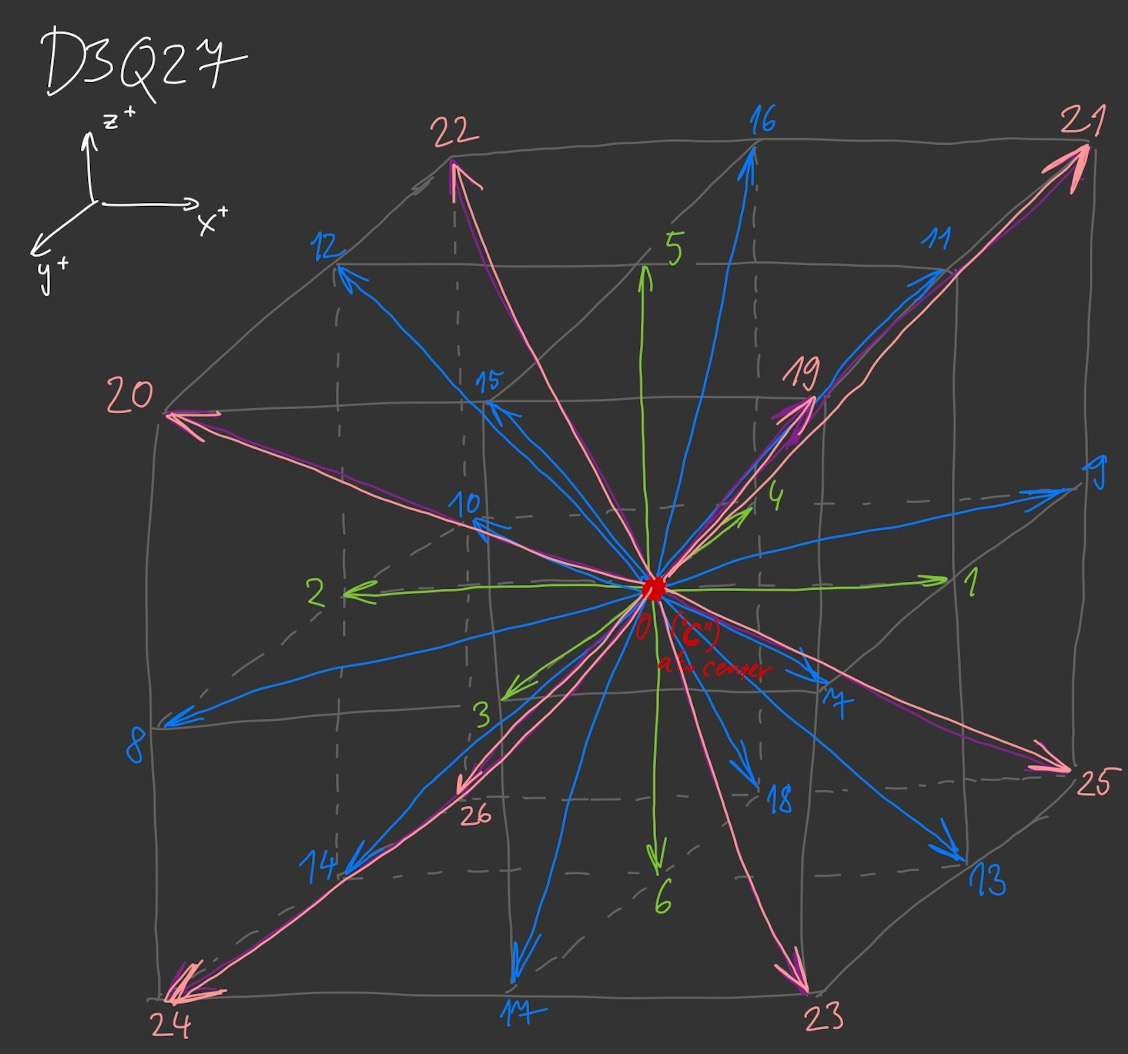
\includegraphics[width=0.4\textwidth]{figures/d3q27-bad.jpg}
%	\caption{D3Q27 node - PREROBIT NA DIAGRAM!!!}
%	\label{fig:d2q27-node}
%\end{figure}

%\begin{equation}
%|f (x_i,t)\rangle = (f_0(x_i,t),f_1(x_i,t),...,f_Q−1(x_i,t)).
%\end{equation}

\begin{equation}
	\label{eq:moments}
	\bm{m} = [m_0, m_1,...,m_{26}]^T
\end{equation}

For better numerical stability, Multiple Relaxation Time (MRT) scheme is used. It allows for more degrees of freedom and better tunability of relaxation parameters. Stability is a key property in any numerical scheme \cite{succi2001lattice}. It helps to protect against cumulative error build-up or other sources of inaccuracies.

Caution have to be taken when working within lattice's discrete world. For simulating the interface of blown oxygen with melted fluid slag, we're working with higher Mach speeds. The basic notion is that the lattice can only support signals with a finite propagation speed. Necessary criterion for stability is that physical information should not travel faster than fastest speed supported by the lattice \cite{succi2001lattice}.

We can calculate the error to $\varepsilon(Ma^3)$ in space and proportional to $\varepsilon (Ma \cdot dt)$ in time, where $Ma = \frac{u}{c_s}$ is the Mach number of the system.

$p = c_s^2 \rho$ is the pressure, $c_s = \frac{c}{\sqrt{3}}$ is the speed of sound, and the kinematic and viscosity $\nu$ is related to the relaxation time rates for the second-order moments by $\nu = \left(\frac{1}{s_v - 0.5}\right) c_s^2 \Delta t$ and $\xi = \frac{2}{3}\left(\frac{1}{s_b - 0.5}\right)$ respectively.

Transformation matrix $\bm{M}$ can be obtained from Eqs. \ref{eq:moments}.

\section{Simulation Software}

\subsection{GPU Computing}

\subsubsection{CUDA and OpenCL}

\subsubsection{ArrayFire}

\subsection{Programming Language}

The Rust programming language helps you write faster, more reliable software. High-level ergonomics and low-level control are often at odds in programming language design; Rust challenges that conflict. Through balancing powerful technical capacity and a great developer experience, Rust gives you the option to control low-level details (such as memory usage) without all the hassle traditionally associated with such control. \cite{steveklabnik2018}

\subsubsection{Why I Chose Rust Programming Language}

Rust is ideal for many people for a variety of reasons.

When 

Rust is for people who crave speed and stability in a language. By speed, we mean the speed of the programs that you can create with Rust and the speed at which Rust lets you write them. The Rust compiler’s checks ensure stability through feature additions and refactoring. This is in contrast to the brittle legacy code in languages without these checks, which developers are often afraid to modify. By striving for zero-cost abstractions, higher-level features that compile to lower-level code as fast as code written manually, Rust endeavors to make safe code be fast code as well. \cite{steveklabnik2018}

The Rust language hopes to support many other users as well; those mentioned here are merely some of the biggest stakeholders. Overall, Rust’s greatest ambition is to eliminate the trade-offs that programmers have accepted for decades by providing safety and productivity, speed and ergonomics. Give Rust a try and see if its choices work for you. \cite{steveklabnik2018}

It wasn’t always so clear, but the Rust programming language is fundamentally about empowerment: no matter what kind of code you are writing now, Rust empowers you to reach farther, to program with confidence in a wider variety of domains than you did before.

Take, for example, “systems-level” work that deals with low-level details of memory management, data representation, and concurrency. Traditionally, this realm of programming is seen as arcane, accessible only to a select few who have devoted the necessary years learning to avoid its infamous pitfalls. And even those who practice it do so with caution, lest their code be open to exploits, crashes, or corruption.

Rust breaks down these barriers by eliminating the old pitfalls and providing a friendly, polished set of tools to help you along the way. Programmers who need to “dip down” into lower-level control can do so with Rust, without taking on the customary risk of crashes or security holes, and without having to learn the fine points of a fickle toolchain. Better yet, the language is designed to guide you naturally towards reliable code that is efficient in terms of speed and memory usage.

Programmers who are already working with low-level code can use Rust to raise their ambitions. For example, introducing parallelism in Rust is a relatively low-risk operation: the compiler will catch the classical mistakes for you. And you can tackle more aggressive optimizations in your code with the confidence that you won’t accidentally introduce crashes or vulnerabilities.

But Rust isn’t limited to low-level systems programming. It’s expressive and ergonomic enough to make CLI apps, web servers, and many other kinds of code quite pleasant to write — you’ll find simple examples of both later in the book. Working with Rust allows you to build skills that transfer from one domain to another; you can learn Rust by writing a web app, then apply those same skills to target your Raspberry Pi.

This book fully embraces the potential of Rust to empower its users. It’s a friendly and approachable text intended to help you level up not just your knowledge of Rust, but also your reach and confidence as a programmer in general. So dive in, get ready to learn—and welcome to the Rust community!

\cite{steveklabnik2018}

\section{Visualization Software}

Scientific visualization is the use of computer graphics to create visual images that aid in the understanding of complex numerical representations of scientific concepts or re- sults. Computational fluid dynamics (CFD) based numerical simulations often output massive amounts of data. These simulations often contain high-dimensional data in a three- dimensional volume. The display of phenomena associated with this data may involve complex three-dimensional structures.

\subsection{Human-Computer Interface}

\subsubsection{SCADA}

- ako sa scada systemy pouzivaju

- neexistuje prepojenie s virtualnou realitou

- future work co by sa dalo spravit

\subsection{Visualization Tools}

\subsubsection{The Visualization Toolkit}

\subsubsection{ParaView}

\subsection{Virtual and Augmented Reality}

Non-immersive interactive visualization systems implemented for the conventional desktop and mouse are effective for moderately complex problems. Immersive virtual environments, by comparison, lie at the other end of the spectrum and permit looking around an object by moving one's head position.

Therefore, a fun- damental difference between desktop-and-mouse virtual realia and immersive VR is that the latter is a true 3D representation that may be either viewer or object-centered while the first is exclusively viewer-centered. In other words, changes in the relative positions of a 2D object’s components result from shifts in the viewer’s perspective. The same may be true for objects viewed in a three dimensional environment, whether real or vir- tual. However, in such an environment, an object may also appear to change shape (e.g., through foreshortening), not due to an altered position of the viewer, but because the ob- ject itself has moved to a different position. Immersive virtual reality displays aid in the unambiguous display of these structures by providing a rich set of spatial and depth cues. Virtual reality interface concepts allow the rapid and intuitive exploration of the volume containing the data, enabling the phenomena at various places in the volume to be ex- plored, as well as provide simple control of the visualization environment through inter- faces integrated into the environment (Bryson; 1996).

Desktop-and-mouse interfaces for 3D visualizations make it difficult to specify positions in three dimensions and do not provide unambiguous display of 3D structure. Virtual reality interfaces attempt to provide the most anthropomorphic interfaces possible - that means they must be human-conforming and should be designed to allow the most natural, unambiguous way of scientific exploration. They must include two components: display and user control. Scientific visualization makes particular demands on virtual reality displays. The phenomena to be displayed in a scientific visualization application often involve delicate and detailed structure, requiring high-quality, high-resolution full-color displays. A wide field of view is often desirable, because it allows the researcher to view how detailed structures are related to larger, more global phenomena.

Historically, the early attempts at using head-mounted virtual reality technologies started with CRT-based Binocular Omni-Oriented Monitor (BOOM) created by Fakespace Systems Inc. BOOM was a stereoscopic display device with screens and optical system housed in a box that is attached to a multi-link arm. Head tracking was accomplished via sensors in the links of the arm that holds the box.

Advent of commodity-level VR hardware like HTC Vive or Oculus Touch has made this technology accessible for meaningful applications. These headset utilize lasers and photosensitive sensors (HTC Vive) or cameras (Oculus Touch) for head and hands tracking and provide six degrees of freedom (6DoF) for movement in virtual environment. By immersing the user into the simulation itself, virtual reality reveals the spatially complex structures in computational science in a way that makes them easy to understand and study. But beyond adding a 3D interface, virtual reality also means greater computational complexity (Bryson; 1996). The ability to provide real-time interaction can provide strong depth cues, either through allowing interactive rotations or through the use of head-tracked rendering. Applications and techniques are being developed to discern how immersive technology benefits visualization. The medical field provides an especially promising context for this development, as medical practitioners require a thorough understanding of specific 3D structures: human anatomy. Users may interact simultaneously with high resolution computed tomography (CT) scans and their corresponding, 3D anatomical structures.

Another frequently used type of immersive, interactive display technology nowadays is projection-screen-based Cave Automatic Virtual Environment (CAVE). These systems consists of 3 to 6 large displays positioned into a room-sized cube around the observer. The walls of a CAVE are typically made up of rear-projection screens, but recently the flat panel displays are commonly used. The floor can be a downward-projection screen, a bottom projected screen or a flat panel display. The projection systems are very high-resolution due to the near distance viewing which requires very small pixel sizes to retain the illusion of reality. The user wears 3D glasses inside the CAVE to see 3D graphics generated by the CAVE. People using the CAVE can see objects apparently floating in the air, and can walk around them, getting a proper view of what they would look like in reality. This is made possible by infrared cameras. Movement of the observer in the CAVE is tracked by the sensors typically attached to the 3D glasses and the video continually adjusts to retain the viewers perspective.

Many universities and engineering companies own and use CAVE systems. Researchers can use these systems to conduct their research topic in a more effective and accessible method. Engineers have found them useful in enhancing of a product development through prototyping and testing phases.

In field of mathematics, VR application named Cal (2019) is making serious progress. It is developed by a company Nanome, Inc. started by students from University of California San Diego. Team behind Calcflow is using VR to help students grasp the biggest ideas in vector calculus. Its features include visualizations of vector addition, cross product, parametrized functions, spherical coordinate mapping, double and surface integrals. Beside Calcflow, they are implementing a VR platform specialized for atomic, molecular and protein visualization, built for researchers and scientists (Nan; 2019).

One can say that virtual reality established itself in many disciplines of human activities, as a medium that allows easier perception of data or natural phenomena appearance. In fact, theme of this dissertation was influenced by my previous work with using virtual reality for mathematics education at the university TODO: CITOVAT MATHWORLDVR CLANOK!!!

\subsubsection{Virtual Reality in Steelmaking}

Substantial amount of work in applying 3D visualizations and virtual reality for solving technological issues and bringing new trends into steelmaking industry is currently happening at Center for Innovation through Visualization and Simulation (CIVS) at Purdue University Northwest (located in Indiana, USA). CIVS has been globally recognized for its integrated and application-driven approaches through state-of-the-art simulation and virtual reality visualization technologies for providing innovative solutions to solve various university research problems, industry issues, as well as education. More than 350 projects that have been completed at the center from its inception in 2014 until today provided substantial educational and economic impact, resulting in more than 40 million US dollars (more than 36.1 million e at the time of this writing) in savings for companies. In collaboration with other universities and companies from steelmaking industry, they focus on research regarding integration of virtual reality with simulation technologies and high performance computing; application of simulation and visualization technologies to industrial processes for process design trouble-shooting and optimization to address the issues of productivity, energy, environment, and quality; and last but not least, development of advanced learning environments in virtual reality for training and education. They launched novel, industry-led association of steel manufacturers and stakeholders called Steel Manufacturing Simulation and Visualization Consortium (SMSVC).

Interesting application of combining 3D CFD smulation and virtual reality for visual in- spection is pulverized coal injection (PCI) and coke combustion model. Research efforts between the Canadian government (CANMET), CIVS and the American Iron and Steel Institute (AISI) were conducted and resulted in modeling of the blowpipe and tuyere of the blast furnace. Combination of aforementioned technologies turned out to be powerful and provided detailed information of flow streams that were previously very difficult to measure. The CFD model shown in Fig. 2 – 12 was used to simulate PCI with natural gas co-injection in the lance, blowpipe and tuyere TODO: DOPLNIT CITACIU!!!.

Another very interesting project conducted at CIVS involved development of compre- hensive package of modules for simulating multiple processes in blast furnace. 3D CFD model shown in Fig. 2 – 13 has been developed by Zheng and Hu (2014) specifically for simulating the blast furnace hearth. The campaign life of a blast furnace is highly dependent on residual thickness of refractory lining in the hearth. The progress of hearth lining erosion is greatly affected by hot metal flow patterns and heat transfer in refractory under different operating conditions. CFD model incorporates both the hot metal flow and conjugate heat transfer through the refractories. They achieved consistency of results between measured and calculated refractory temperature profiles, as the model has been extensively validated using measurement data from industry blast furnace. The virtual reality (VR) visualization technology has been used to analyze the velocity and temperature distributions and wear patterns of different furnaces and operating conditions. This interactive 3D visualization is shown in Fig. 2 – 14. Based on the results, it was possible to predict the inner profile of hearth and provide guidance to protecting the blast furnace hearth.

\subsection{Visualizing Simulation in Virtual Reality}

\section{Results}

\section{Conclusions}

\section{Discussion}

\section{Appendix A: Simulation as an Educational Tool}

In some simplified form, combinations of numerical simulations and visualizations of steel- making processes can be used as a educational tool in process control courses at technical universities. The aim of the online, web-based interactive simulation of basic oxygen steelmaking at steeluniversity.org shown in Fig. \ref{fig:steeluniversity} is to introduce students to this process in a more fun and engaging way.

\begin{figure}[!ht]
	\label{fig:steeluniversity}
	\centering
	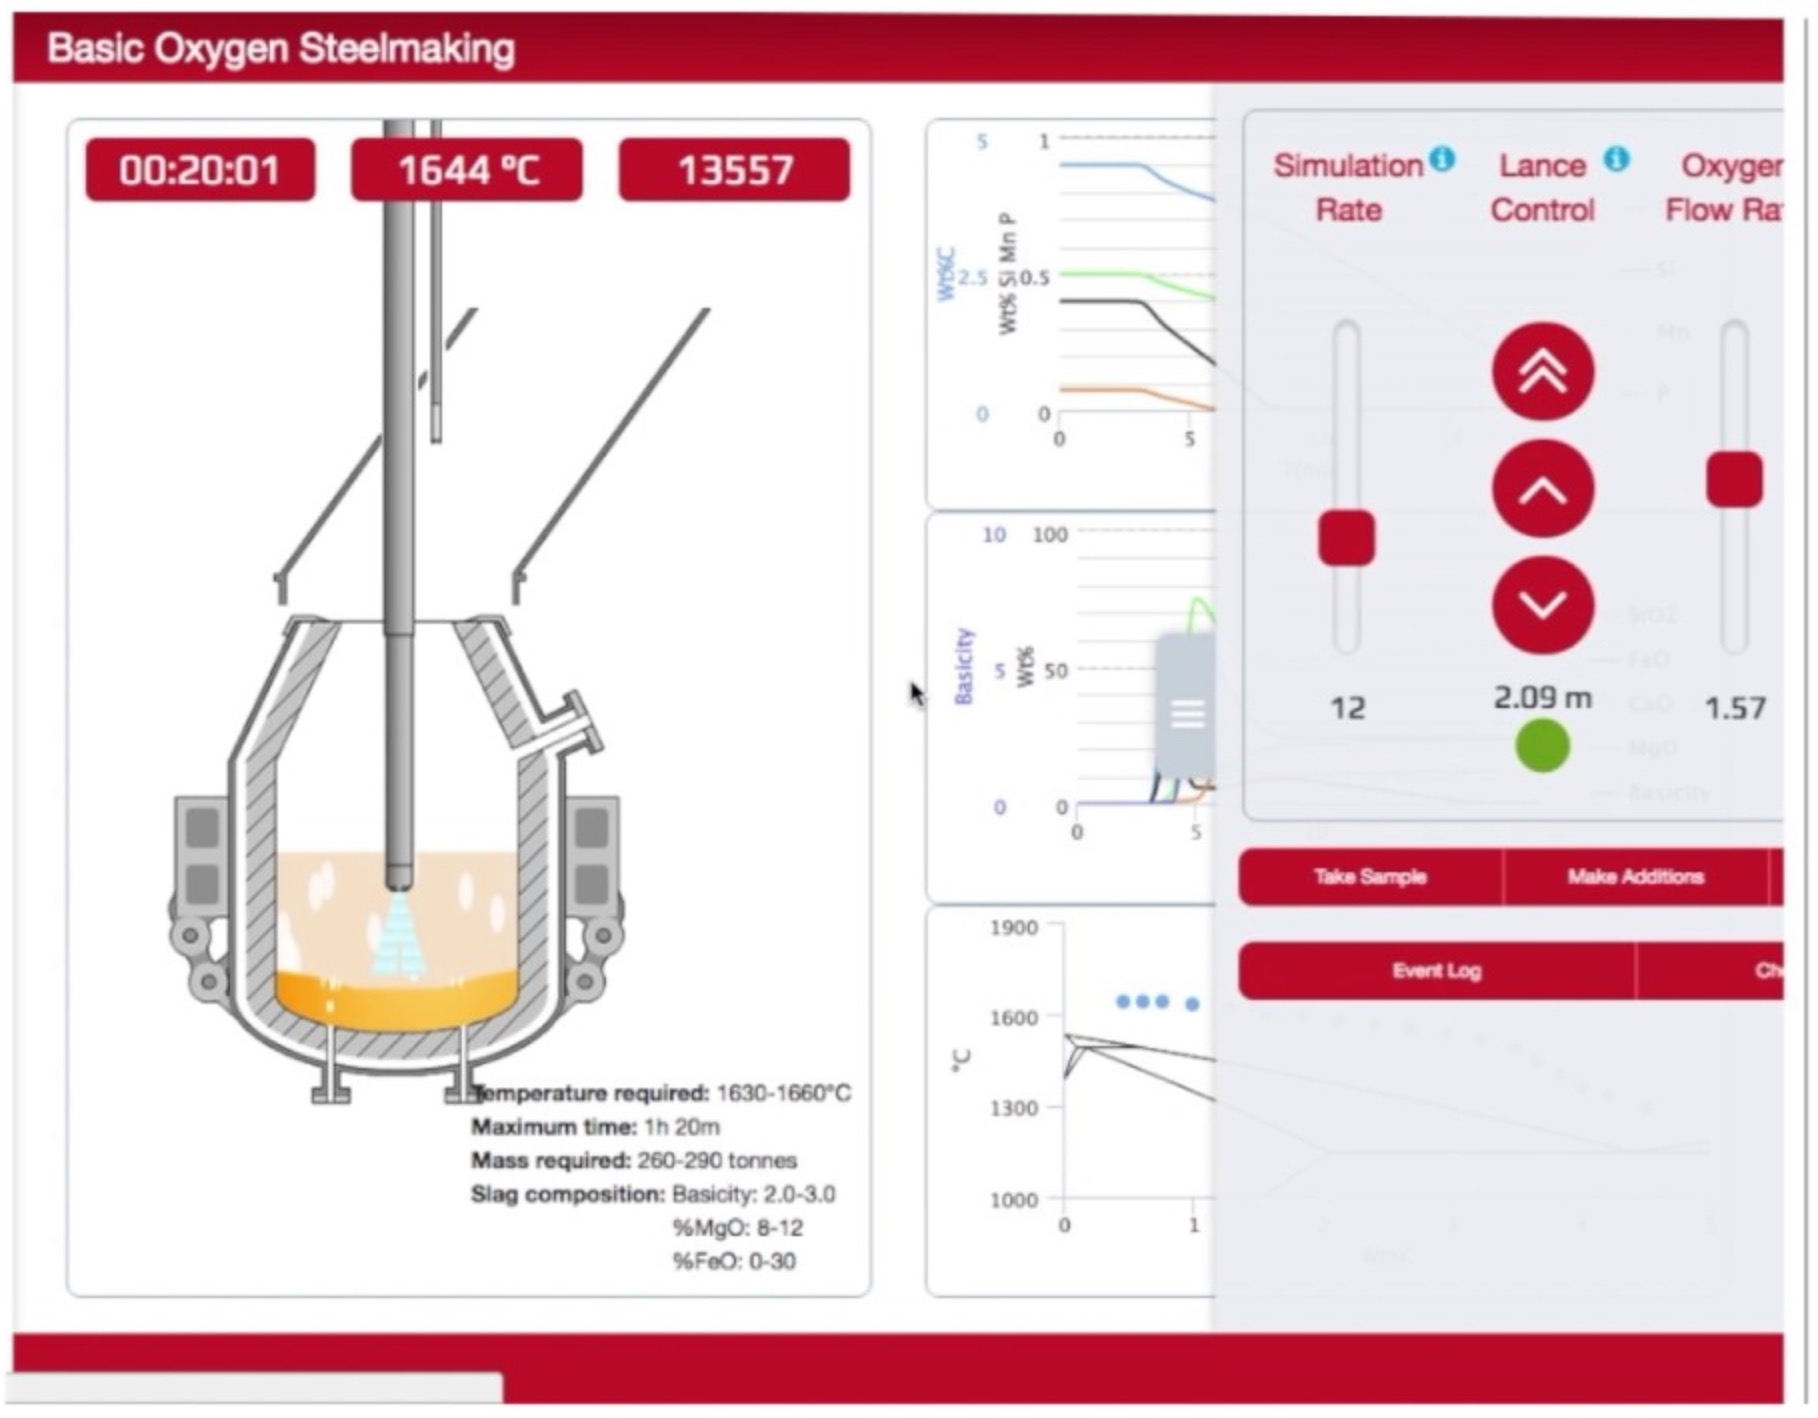
\includegraphics[width=0.8\textwidth]{figures/steeluniversity.jpg}
	\caption{Interactive, educational simulation of basic oxygen steelmaking by steeluniversity.org.}
\end{figure}
%
%%
\Urlmuskip=0mu plus 1mu\relax
\bibliographystyle{spbasic}
\bibliography{refs/control,refs/mathematics,refs/modeling,refs/cfd,refs/lbm,refs/gpu,refs/interaction,refs/interfaces,refs/hci,refs/design,refs/ml,refs/visualization,refs/programming,refs/simulation,refs/ar,refs/vr,refs/online}

%
\section*{Appendices}
\addcontentsline{toc}{section}{\numberline{}Appendices}
\thispagestyle{empty}

\begin{description}
	\item[Appendix A] System Manual
	\item[Appendix B] User Manual
\end{description}
%
\section*{Appendix A}
\addcontentsline{toc}{section}{\numberline{}Appendix A}
%%
\subsection*{System Manual}

\subsubsection*{Hardware Requirements}

TODO: \\

Hardware requirements (PC, VR) \\

\begin{table}[!ht]
	\centering\footnotesize
	\begin{tabular}{ |p{4cm}||p{5.1cm}|p{5.1cm}|  }
		\hline
		Component & Recommended Specs & Minimum Specs \\
		\hline
		Processor & Intel i5-4590 / AMD Ryzen 5 1500X or greater & Intel i3-6100 / AMD Ryzen 3 1200, FX4350 or greater  \\
		Graphics Card & NVIDIA GTX 1060 / AMD Radeon RX 480 or greater & NVIDIA GTX 1050 Ti / AMD Radeon RX 470 or greater  \\
		Alternative Graphics Card & NVIDIA GTX 970 / AMD Radeon R9 290 or greater & NVIDIA GTX 960 4GB / AMD Radeon R9 290 or greater  \\
		Memory & 8GB+ RAM & 8GB+ RAM  \\
		Operating System & Windows 10 & Windows 10  \\
		USB Ports & 3x USB 3.0 ports, plus 1x USB 2.0 port & 1x USB 3.0 port, plus 2x USB 2.0 ports  \\
		Video Output & 	Compatible HDMI 1.3 video output & Compatible HDMI 1.3 video output  \\
		\hline
	\end{tabular}
	\caption{Hardware specifications for VR support.}
	\label{tab:vr-specs}
\end{table}

Windows 10 is the minimum supported operating system because Microsoft stopped supporting the Windows 7 and 8.1, beginning from 14th of January 2020.
%
\section*{Appendix B}
\addcontentsline{toc}{section}{\numberline{}Appendix B}
%\appendix
%\section{Príloha}
\subsection*{Bibliografick\'e odkazy}

Táto časť\/ záverečnej práce je povinná. V~zozname použitej literatúry
sa uvádzajú odkazy podľa normy STN ISO 690--2 (01 0197) (Informácie
a~dokumentácia. Bibliografické citácie. Časť\/ 2: Elektronické
dokumenty alebo ich časti, dátum vydania 1.~12.~2001, ICS: 01.140.20).
Odkazy sa môžu týkať\/ knižných, časopiseckých a~iných zdrojov
informácií (zborníky z~konferencií, patentové dokumenty, normy,
odporúčania, kvalifikačné práce, osobná korešpondencia a~rukopisy,
odkazy cez sprostredkujúci zdroj, elektronické publikácie), ktoré boli
v~záverečnej práci použité.

Forma citácií sa zabezpečuje niektorou z~metód, opísaných v~norme STN
ISO 690, 1998, s.~21. Podrobnejšie informácie nájdete na stránke
\texttt{http://www.tuke.sk/anta/} v~záložke {\small\sf Výsledky
práce/Prehľad normy pre publikovanie STN ISO 690 a~STN ISO 690-2}.

Existujú dva hlavné spôsoby citovania v~texte.

\begin{itemize}
\item Citovanie podľa mena a~dátumu.
\item Citovanie podľa odkazového čísla.
\end{itemize}

\emph{Preferovanou metódou citovania} v~texte vysokoškolskej
a~kvalifikačnej práce je podľa normy ISO 7144 citovanie podľa mena
a~dátumu \citep{kat,gonda}. V~tomto prípade sa zoznam použitej
literatúry upraví tak, že za meno sa pridá rok vydania. Na uľahčenie
vyhľadávania citácií sa zoznam vytvára v~abecednom poradí autorov.

\medskip

Príklad:
\dots podľa \citep{steinerova} je táto metóda dostatočne rozpracovaná
na to, aby mohla byť\/ všeobecne používaná v~\dots

\medskip

Druhý spôsob uvedenia odkazu na použitú literatúru je uvedenie len
čísla tohto zdroja v~hranatých zátvorkách bez mena autora (autorov)
najčastejšie na konci príslušnej vety alebo odstavca.

\medskip

Príklad:
\dots podľa [13] je táto metóda dostatočne rozpracovaná na to, aby
mohla byť\/ všeobecne používaná v~\dots ako je uvedené v~[14].

\medskip

Citácie sú spojené s~bibliografickým odkazom poradovým číslom v~tvare
indexu alebo čísla v~hranatých zátvorkách. Odkazy v~zozname na konci
práce budú usporiadané podľa týchto poradových čísel. Viacero citácií
toho istého diela bude mať\/ rovnaké číslo. Odporúča sa usporiadať\/
jednotlivé položky v~poradí citovania alebo podľa abecedy.

\medskip
\noindent
Rôzne spôsoby odkazov je možné dosiahnuť\/ zmenou voľby v~balíku
\verb+natbib+:

\noindent
\verb+% Citovanie podla mena autora a roku+\\
\verb+\usepackage[]{natbib}\citestyle{chicago}+\\
\verb+% Možnosť rôznych štýlov citácií. Príklady sú uvedené+\\
\verb+% v preambule súboru natbib.sty.+\\
\verb+% Napr. štýly chicago, egs, pass, anngeo, nlinproc produkujú+\\
\verb+% odkaz v tvare (Jones, 1961; Baker, 1952). V prípade, keď+\\
\verb+% neuvedieme štýl citácie (vynecháme \citestyle{}) v "options"+\\
\verb+% balíka natbib zapíšeme voľbu "colon".+

\medskip
\noindent
Keď zapneme voľbu \verb+numbers+, prepneme sa do režimu citovania
podľa odkazového čísla.

\noindent
\verb+% Metoda ciselnych citacii+\\
\verb+\usepackage[numbers]{natbib}+

\bigskip

Pri zápise odkazov sa používajú nasledujúce pravidlá:

V~odkaze na knižnú publikáciu (pozri príklad zoznamov na konci tejto
časti):
\begin{itemize}
\item Uvádzame jedno, dve alebo tri prvé mená oddelené pomlčkou,
ostatné vynecháme a~namiesto nich napíšeme skratku et al. alebo a~i.
\item Podnázov sa môže zapísať\/ vtedy, ak to uľahčí identifikáciu
dokumentu. Od názvu sa oddeľuje dvojbodkou a~medzerou.
\item Dlhý názov sa môže skrátiť\/ v~prípade, ak sa tým nestratí
podstatná informácia. Nikdy sa neskracuje začiatok názvu. Všetky
vynechávky treba označiť\/ znamienkami vypustenia  \dots
\end{itemize}

Pri využívaní informácií z~elektronických dokumentov  treba
dodržiavať\/ tieto zásady:
\begin{itemize}
\item  uprednostňujeme autorizované súbory solídnych služieb
a~systémov,
\item zaznamenáme dostatok informácií o~súbore tak, aby ho bolo opäť\/
možné vyhľadať\/,
\item urobíme si kópiu použitého prameňa v~elektronickej alebo
papierovej forme,
\item za verifikovateľnosť\/ informácií zodpovedá autor, ktorý sa na
ne odvoláva.
\end{itemize}

Pre zápis elektronických dokumentov platia tie isté pravidlá, ako pre
zápis klasických. Navyše treba uviesť\/ tieto údaje:
\begin{itemize}
\item  druh nosiča  [online], [CD-ROM], [disketa], [magnetická páska]
\item dátum citovania  (len pre online dokumenty)
\item dostupnosť\/  (len pre online dokumenty)
\end{itemize}

Poradie prvkov odkazu je nasledovné:
Autor. Názov. In Názov primárneho zdroja: Podnázov. [Druh  nosiča].
Editor. Vydanie alebo verzia. Miesto vydania : Vydavateľ, dátum
vydania. [Dátum citovania]. Poznámky.  Dostupnosť\/. ISBN alebo ISSN.
%
%\section*{Appendix C}
\addcontentsline{toc}{section}{\numberline{}Appendix C}
\subsection*{Vytvorenie zoznamu skratiek a symbolov}



%% begin the 'Curriculumvitae' of the author
%\curriculumvitae\protect\label{page:posledna}
%Táto časť\/ je nepovinná. Autor tu môže uviesť\/ svoje biografické
%údaje, údaje o~záujmoch, účasti na~projektoch, účasti na~súťažiach,
%získané ocenenia, zahraničné pobyty na~praxi, domácu prax, publikácie
%a~pod.
%\endcurriculumvitae

\end{document}
%%